%---------------------------------------------------------------------
%
%                          Cap�tulo 4
%
%---------------------------------------------------------------------
%
% 04Imagenes.tex
% Copyright 2009 Marco Antonio Gomez-Martin, Pedro Pablo Gomez-Martin
%
% This file belongs to the TeXiS manual, a LaTeX template for writting
% Thesis and other documents. The complete last TeXiS package can
% be obtained from http://gaia.fdi.ucm.es/projects/texis/
%
% Although the TeXiS template itself is distributed under the 
% conditions of the LaTeX Project Public License
% (http://www.latex-project.org/lppl.txt), the manual content
% uses the CC-BY-SA license that stays that you are free:
%
%    - to share & to copy, distribute and transmit the work
%    - to remix and to adapt the work
%
% under the following conditions:
%
%    - Attribution: you must attribute the work in the manner
%      specified by the author or licensor (but not in any way that
%      suggests that they endorse you or your use of the work).
%    - Share Alike: if you alter, transform, or build upon this
%      work, you may distribute the resulting work only under the
%      same, similar or a compatible license.
%
% The complete license is available in
% http://creativecommons.org/licenses/by-sa/3.0/legalcode
%
%---------------------------------------------------------------------

\chapter{Implementaci\'on de las aplicaciones}
\label{cap4}
\label{cap:impl}

En el cap\'itulo anterior se analizaron las diferentes opciones de dise\~no del proyecto y se detall\'o el protocolo de comunicaci\'on entre el juego y el dispositivo m\'ovil. Adem\'as de esto se expusieron las ventajas y desventajas de usar los diferentes conjuntos de caracter\'isticas expuestas. En este cap\'itulo se detallar\'a todo el proceso de creaci\'on y desarrollo de las diferentes aplicaciones que utilizan el protocolo de comunicaci\'on anteriormente expuesto.\\

Se ha divido este cap\'itulo en 2 secciones, una para cada aplicaci\'on desarrollada:\\

\begin {itemize}
\item Implementaci\'on de la aplicaci\'on de Android (secci\'on \ref{android})
\item Implementaci\'on de la aplicaci\'on de Unity (secci\'on \ref{unity})
\end {itemize}

%-------------------------------------------------------------------
\section{Implementaci\'on de la aplicaci\'on de Android}
\label{android}
%-------------------------------------------------------------------

El objetivo principal de la aplicaci\'on Android es poder utilizar este dispositivo como un mando. Para conseguir esto la aplicaci\'on recibe un flujo de im\'agenes enviadas desde el juego. La aplicaci\'on est\'a restringida a un uso exclusivo en apaisado. Cada vez que la aplicaci\'on registre una pulsaci\'on del usuario en la pantalla, esta enviar\'a por red al juego las coordenadas de la pulsaci\'on. Para poder hacer este env\'io, la aplicaci\'on m\'ovil debe conocer la IP del dispositivo que ejecuta el juego y en qu\'e puerto espera recibir los mensajes. Para evitar que el usuario tenga que escribir estos datos y mejorar la usabilidad de la aplicaci\'on, este proceso se hace con c\'odigos QR. Como se ver\'a m\'as adelante, el juego debe mostrar el c\'odigo QR que codifica la cadena IP:Puerto.\\

En el momento de arranque, la aplicaci\'on activar\'a la c\'amara del dispositivo m\'ovil para que el usuario escanee el c\'odigo QR. Con esto la aplicaci\'on recibe los datos que necesita para iniciar la conexi\'on con el juego sin que el usuario tenga que preocuparse por nada m\'as.\\

%-------------------------------------------------------------------
\subsection {Conceptos b\'asicos de Android}
%-------------------------------------------------------------------



Android Studio es el entorno de desarrollo integrado (IDE) oficial para la plataforma de Android. Actualmente Android Studio est\'a disponible para las plataformas Microsoft Windows, macOS y GNU/Linux. Android Studio incluye una gran variedad de herramientas para facilitar el desarrollo en Android entre las que se incluyen:\\

\begin {itemize}
\item Plantillas para crear dise\~nos comunes de Android y otros componentes.
\item Un editor de dise\~no enriquecido que permite a los usuarios arrastrar y soltar componentes de la interfaz de usuario.
\item Soporte para construcci\'on basada en Gradle.
\item Dispositivos virtuales de Android que se utiliza para ejecutar y probar aplicaciones.
\item Consola de desarrollador: consejos de optimizaci\'on, ayuda para la traducci\'on y estad\'isticas de uso.
\item Integraci\'on de ProGuard y funciones de firma de aplicaciones.
\end {itemize}



Los lenguajes de programaci\'on aceptados por Android Studio son Kotlin, Java y C++. En concreto para este proyecto se ha usado Java como lenguaje de programaci\'on.\\

Android es un sistema operativo que gestiona el ciclo de vida de sus aplicaciones. Las aplicaciones en Android se rigen por una serie de componentes. Uno de estos componentes son las \textbf{\textit{Activity}}. Estos componentes son claves a la hora de manejar los estados de una aplicaci\'on en Android. A diferencia de otros paradigmas de programaci\'on que comienzan sus aplicaciones con un m\'etodo \texttt{main()}, la instancia de una Actividad invoca m\'etodos de devoluci\'on de llamada (\emph{callbacks}) que se corresponden con etapas espec\'ificas de su ciclo de vida. La experiencia de una aplicaci\'on para un dispositivo m\'ovil difiere mucho de la versi\'on de escritorio de esa misma aplicaci\'on ya que la interacci\'on del usuario con la aplicaci\'on no siempre comienza en el mismo lugar. Un claro ejemplo de esto sucede con las aplicaciones de mensajer\'ia instant\'anea. Un usuario puede estar navegando por cualquier red social y encontrarse una publicaci\'on interesante y compartirla por correo electr\'onico o por una aplicaci\'on de mensajer\'ia instant\'anea.\\

 \begin{figure}[!h]
    \centering
    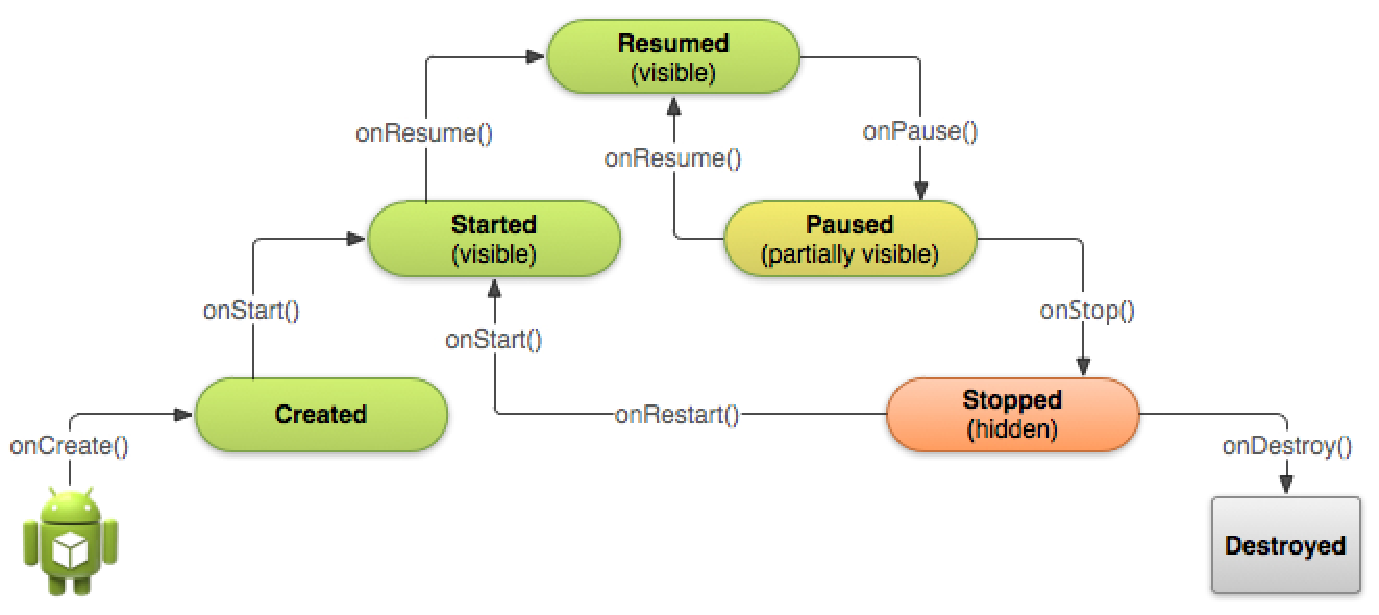
\includegraphics[width=0.90\textwidth]{./Imagenes/Vectorial/lifecycle-states.pdf}
    \caption{Estados de las aplicaciones Android}
\label{Fig:estados}
\end{figure}

La mayor\'ia de las aplicaciones contienen varias pantallas, lo cual significa que contienen varias actividades. Este concepto se pondr\'a posteriormente de manifiesto ya que para el desarrollo de la aplicaci\'on han sido necesarias dos Actividades.
Cuando un usuario navega por una aplicaci\'on, la cierra, la vuelve a abrir o la minimiza, las instancias de las Actividades de la aplicaci\'on pasan por una serie de estados de su ciclo de vida (figura \ref{Fig:estados}).\footnote{\url{https://rb.gy/atkae1}} Estos estados son controlados por el propio sistema Android. Cuando la aplicaci\'on cambia de estado, el sistema avisa a la Actividad mediante los siguientes \emph{callbacks}: \textbf{onCreate(), onStart(), onResume(), onPause(), onStop() y onDestroy()} (figura~\ref{ciclo}).\footnote{\url{https://rb.gy/py2et6}}\\

\begin{figure}[h]

\centering
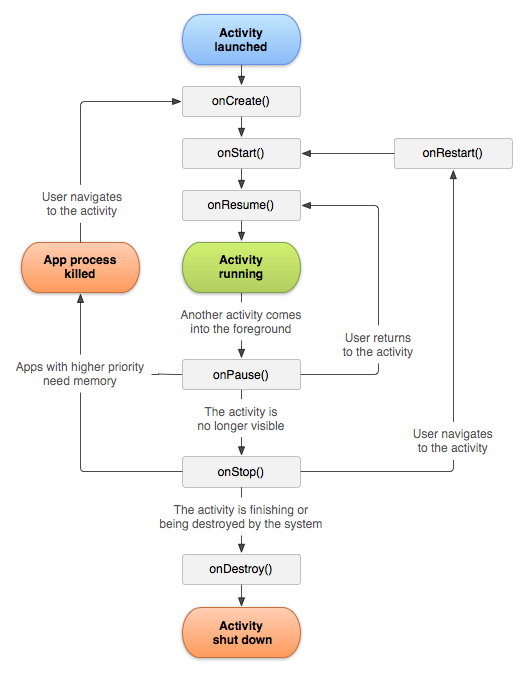
\includegraphics[width=0.7\textwidth]{./Imagenes/Bitmap/Ciclo_de_vida_Android}
\caption{Ciclo de vida de una Actividad de un sistema Android}
\label{ciclo}
\end{figure}

Cada uno de los \emph{callbacks} que tiene la actividad es llamado en un momento concreto de la ejecuci\'on de la Actividad. Las caracter\'isticas de cada una de estas llamadas son las siguientes:\\

\begin {itemize}
\item \textbf{onCreate()} $\rightarrow$ Este m\'etodo es el primero que llama cuando se crea la Actividad. Este estado es utilizado para ejecutar la l\'ogica de la aplicaci\'on que debe ocurrir \'unicamente una vez en todo el ciclo de vida.
\item \textbf{onStart()} $\rightarrow$ Cuando la actividad entra en el estado Started, el sistema invoca esta devoluci\'on de llamada. La llamada \textit{onStart()} hace que el usuario pueda ver la actividad mientras la app se prepara para entrar en primer plano y se convierta en interactiva.
\item \textbf{onResume()} $\rightarrow$  El sistema invoca esta devoluci\'on de llamada cuando una Actividad que estaba pausada vuelve a ser el foco.
\item \textbf{onPause()} $\rightarrow$ Esta devoluci\'on de llamada es invocada cuando el usuario abandona la Actividad. 
\item \textbf{onStop()} $\rightarrow$ El sistema invoca esa devoluci\'on de llamada una vez la Actividad est\'a a punto de finalizar. En este m\'etodo la aplicaci\'on debe liberar los recursos que no son necesarios mientras esta no sea visible para el usuario.
\item \textbf{onDestroy()} $\rightarrow$ Se llama a este m\'etodo antes de que se finalice la actividad. El sistema invoca esta devoluci\'on de llamada cuando la aplicaci\'on se cierra. En este momento es donde los componentes del ciclo de vida pueden guardar cualquier elemento que se necesite antes de que finalice la Actividad. 
\end {itemize}

En el siguiente apartado se explicar\'a el uso de estas llamadas del sistema Android dentro del proyecto y la utilizaci\'on de diferentes actividades. Adem\'as se expondr\'a la arquitectura de la aplicaci\'on desarrollada para Android.\\


%-------------------------------------------------------------------
\subsection {Desarrollo de la aplicaci\'on Android}
%-------------------------------------------------------------------

Para que la aplicaci\'on Android cumpla los requisitos expuestos en el apartado de especificaci\'on del proyecto, se han implementado 4 clases:\\

\begin {itemize}
\item \textbf{MainActivity} $\rightarrow$ Esta primera clase corresponde a la primera actividad. En esta primera actividad se utiliza la c\'amara para leer un c\'odigo QR y guardar como par\'ametro el contenido del c\'odigo. Este contenido es la IP del equipo donde se est\'a ejecutando el juego y el puerto al que deben ser enviadas las pulsaciones del usuario. Estos datos son pasados a la actividad hija para comenzar a usar el m\'ovil como dispositivo de entrada.
\item \textbf{ControllerActivity} $\rightarrow$ Esta es la actividad principal. Desde esta actividad se recogen los datos de IP y puerto al que debe conectarse el dispositivo Android gracias a la lectura de un c\'odigo QR realizada con la actividad padre. Al crearse la actividad se lanza la ejecuci\'on de una hebra que se encargar\'a de recibir, leer e interpretar las im\'agenes que lleguen por red una vez la aplicaci\'on se conecte al juego. Desde esta clase se controla la pulsaci\'on del usuario en la pantalla. De esta pulsaci\'on se guardan 3 datos: posici\'on (x,y) donde se ha realizado la pulsaci\'on y el tipo de pulsaci\'on (presionar, levantar o arrastrar). Este dato permite soportar el \textit{multitouch} en la aplicaci\'on. El comportamiento de este hilo viene dado en la clase \textbf{UdpClientThread} que se encarga de preparar el datagrama de la pulsaci\'on y enviarlo. La \'ultima funci\'on de esta clase es la de cambiar la imagen que se muestra en la aplicaci\'on. 
\begin{figure}[!h]

\centering
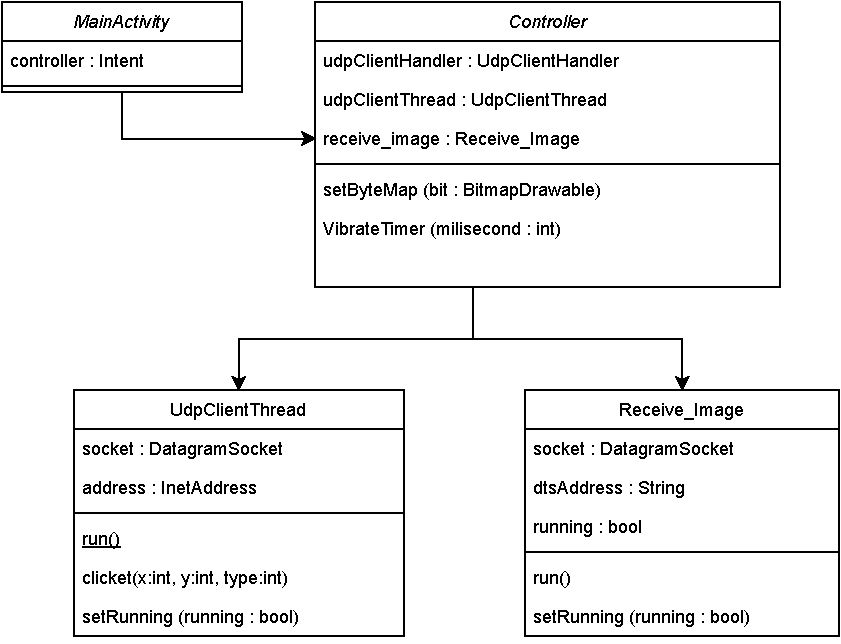
\includegraphics[width=0.85\textwidth]{./Imagenes/Vectorial/Arquitectura_App_Android.pdf}
\caption{Diagrama de clases de la aplicaci\'on Android}
\end{figure}

\item \textbf{UdpClientThread} $\rightarrow$ Esta clase tiene como funci\'on el env\'io de datos a la aplicaci\'on donde se ejecuta el juego. Esta hebra se encarga del env\'io de paquetes que incluyen el tipo de pulsaci\'on que se ha realizado, la coordenada \textit{x} y la coordenada \textit{y} de la pantalla del dispositivo donde se ha realizado la pulsaci\'on.Justo antes del cierre de la aplicaci\'on, el datagrama de cierre de conexi\'on se env\'ia desde esta hebra.

\item \textbf{ReceiveData} $\rightarrow$ Esta clase se ejecuta desde una hebra distinta a la de la Actividad principal y la funci\'on que desempe\~na es la de recibir informaci\'on que mande el juego. En este hilo se espera la llegada del \textit{streaming} de im\'agenes desde el juego. Estas im\'agenes se esperan en formato PNG ya que se realiza la descompresi\'on de este formato. El tiempo de vibraci\'on puede ser modificado en cualquier momento por el desarrollador por lo que ese mensaje tambi\'en es tratado en este hilo.
\end {itemize}




%-------------------------------------------------------------------
\section{Implementaci\'on de la aplicaci\'on de Unity}
\label{unity}
%-------------------------------------------------------------------

Como se coment\'o al principio de este cap\'itulo, el motor de videojuegos elegido para la realizaci\'on de este proyecto ha sido Unity. Unity es un motor de videojuegos multiplataforma creado por \textit{Unity Technologies} en 2005. Unity est\'a disponible como plataforma de desarrollo para Microsoft, Mac OS y Linux y tiene soporte de compilaci\'on con m\'ultiples plataformas:\\

\begin {itemize}
\item \textbf{Web} $\rightarrow$ WebGL.
\item \textbf{PC} $\rightarrow$ Windows, SteamOS, Linux, OS X y Windows Store Apps.
\item \textbf{Dispositivos m\'oviles} $\rightarrow$ iOS, Android, Windows Phone.
\item \textbf{Smart TV} $\rightarrow$ tvOS, Samsung Smart TV, Android TV.
\item \textbf{Consolas} $\rightarrow$ PlayStation Vita, PlayStation 4, Xbox 360, Xbox One, Wii U, Nintendo 3DS, Nintendo Switch.
\item \textbf{Dispositivos de realidad virtual} $\rightarrow$ Oculus Rift, Google Cardboard, HTC Vive, PlayStation VR, Samsung Gear VR
\end {itemize}

Actualmente en la versi\'on 2021.1 de la documentaci\'on de Unity, no existe soporte para la nueva generaci\'on de consolas.\\


%-------------------------------------------------------------------
\subsection {Funcionamiento de Unity}
%-------------------------------------------------------------------

Unity es un motor de videojuegos que aglutina una gran variedad de herramientas para el desarrollo. Estas herramientas van desde inclusiones de \textbf{Scripts} para dar comportamientos espec\'ificos a cada una de las \textbf{Entidades} del juego hasta elementos m\'as visuales como diagramas de estado para el control de las animaciones de un modelo. Para que todos estos sistemas tan diferentes puedan convivir, hay una serie de funciones que se ejecutan en un orden determinado. Unity a su vez se compone de varios elementos clave:\\

\begin {itemize}
\item \textbf{Escena} $\rightarrow$  Las escenas contienen los objetos del juego. Pueden usarse para crear niveles, men\'us o cualquier estado del juego.
\item \textbf{GameObjects / Entidades} $\rightarrow$ Cada una de las escenas contiene objetos. Estos objetos se llaman GameObjects. Cualquier elemento es considerado un GameObject, no tiene por qu\'e tener una representaci\'on visual (m\'usica, c\'amara, etc).
\item \textbf{Componentes} $\rightarrow$ Los componentes son los diferentes atributos que se le dan a los GameObjects para que tengan funcionalidad (movimiento, posici\'on, animaci\'on, colisi\'on f\'isica, etc).
\end {itemize}

Unity ofrece una serie de componentes que dan una funcionalidad ya definida a un objeto, esta funcionalidad va desde tener una posici\'on definida en el mundo hasta emitir un sonido y realizar una animaci\'on. Los desarrolladores pueden programar sus propios componentes usando Scipts. Estos scripts indican a las diferentes entidades c\'omo comportarse. El lenguaje seleccionado para este sistema de \textit{scripting} es C\# y un script debe estar vinculado a una entidad para que este se ejecute. \\

%-------------------------------------------------------------------
\subsection {Desarrollo de la API en Unity}
%-------------------------------------------------------------------

Las caracter\'isticas espec\'ificas de Unity deben tenerse en cuenta para la integraci\'on de la librer\'ia dentro del motor pero la librer\'ia est\'a desarrollada en .NET. El inicio de la comunicaci\'on entre en juego y  el m\'ovil se realiza con la lectura de un QR que lleva los datos de IP del PC donde se est\'a ejecutando el juego y el puerto donde el juego va a estar escuchando y por donde llegar\'an los datos del m\'ovil. Este c\'odigo se genera utilizando la librer\'ia \textbf{ZXing}\footnote{https://archive.codeplex.com/?p=zxingnet} en su versi\'on de .NET. \\

Para que la aplicaci\'on desarrollada en Unity cumpla los requisitos expuestos en el apartado de especificaci\'on del proyecto, se han realizado 2 clases:\\

\begin {itemize}
\item \textbf{UDPSocket} $\rightarrow$ Esta clase se utiliza para la creaci\'on de todo lo necesario para hacer funcionar esta herramienta. Con el m\'etodo \textbf{init()} se inician 2 hebras de ejecuci\'on diferentes. Una de ellas se encarga de enviar los datos necesarios al m\'ovil. Estos datos son tanto la solicitud de vibraci\'on como la imagen a renderizar en el dispositivo o los mensajes de tipo \textit{keepalive} en caso de que el usuario no interact\'ue con el juego en un tiempo determinado. La otra se encarga de recibir los datos de entrada del dispositivo y avisar a los diferentes \textit{listeners}. Estos listeners utilizan esa informaci\'on para los prop\'ositos designados por el desarrollador del juego (mover al personaje, pausar el juego, salir, etc). Esta clase tambi\'en se encarga de cerrar la conexi\'on.

\item \textbf{InputMobileInterface} $\rightarrow$ El desarrollador del juego debe crear una clase que implemente este interfaz. En esta clase se recibir\'an las notificaciones de los eventos que lleguen desde el m\'ovil. Estos eventos son las coordenadas de las pulsaciones, las dimensiones del m\'ovil y el aviso del cierre de la conexi\'on por parte del m\'ovil.
\end {itemize}

\begin{figure}[h]

\centering
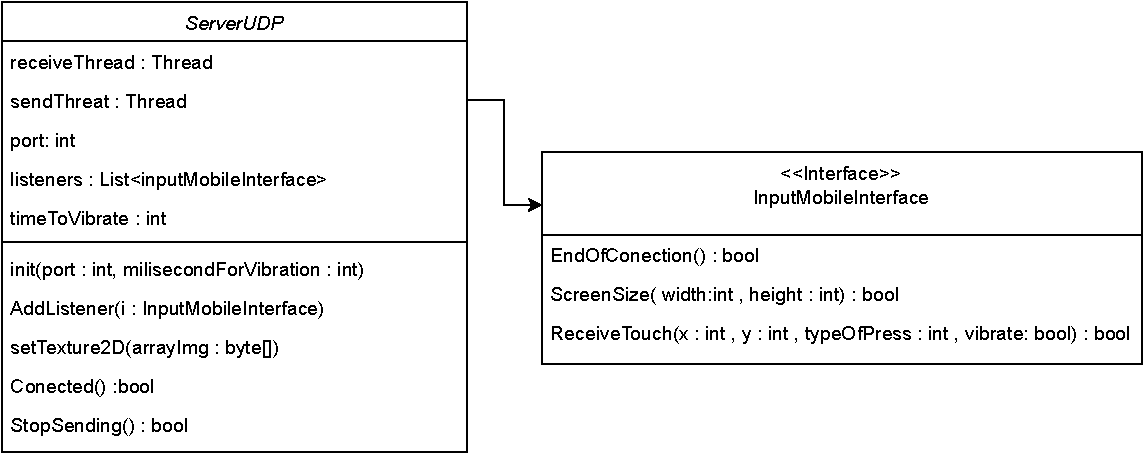
\includegraphics[width=1.0\textwidth]{./Imagenes/Vectorial/Arquitectura Unity.pdf}
\caption{Diagrama de clases de la aplicaci\'on de Unity}
\end{figure}

\vspace{10mm}

\bigskip
\Large{\textbf{En el pr\'oximo cap\'itulo}}\\
\normalsize

En este cap\'itulo se ha expuesto el desarrollo de las aplicaciones de Android y Unity. Adem\'as, se han explicado algunos de los conocimientos b\'asicos para usar ambas herramientas. En el pr\'oximo cap\'itulo se explicar\'a la integraci\'on de la librer\'ia en un juego ya terminado con el que se realizar\'an una serie de pruebas con usuarios. Estas pruebas servir\'an para obtener datos del rendimiento del proyecto. Aplicando una serie de baremos se determinar\'a si el uso de la librer\'ia desarrollada cumple con las expectativas.\\

% Variable local para emacs, para  que encuentre el fichero maestro de
% compilaci�n y funcionen mejor algunas teclas r�pidas de AucTeX
%%%
%%% Local Variables:
%%% mode: latex
%%% TeX-master: "../ManualTeXiS.tex"
%%% End:
